\section {Game Rules}
\label{game-rules}

\begin{enumerate}
\item The game that will be played is called \textbf{QuacMan}.  The aim of the game is for robots to collect as many tokens and ducks as possible.
\item The arena will contain 46 tokens.  They will be arranged in a grid, as shown in figure~\ref{fig:token-arrangement}.  8 of these tokens will be blue\footnote{In the event of tie-breaks (or if the judges get bored), the number of blue tokens in the arena may be increased (and the number of red reduced).}, and the rest will be red.  The arrangement of token colours will be random.
\item There will be a ramp in the middle of the arena.  There is a plastic duck at the top of the ramp.
\item Teams will be assigned a corner of the arena that their robot will start the game in.  The robot must be placed within 100mm of both of the arena walls.
\item At the end of a match, after all tokens have settled, a team's ``\textbf{game points}'' will be counted.
 These are used to rank teams before competition league points are awarded.

\item Game points are awarded as follows:
\begin{itemize}
\item Red tokens collected are worth 1 game point.
\item Blue tokens collected are worth -5 game points.
\item The duck is worth 100 game points.
\end{itemize}

\item At the end of a game, the team with the \emph{most} game points is awarded 4 points towards the competition league.
 The team with the second most is awarded 3.
 The team with the third most is awarded 2 points, and the team with the fewest game points is awarded 1 point.
 Teams whose robot was not entered into the round, or who were disqualified from the round, will be awarded no points.

\item There will be a maximum of 4 robots in a match.
\item A match lasts 180 seconds.
\item Matches are started and stopped by the Student Robotics radio system\footnote{The Student Robotics radio system is supplied as part of the kit.
 It is part of the power board, and is used for safety cut-off, start-match and stop-match signals.}.
\item Teams that do not present their robot promptly for a match will forfeit that match.
\end{enumerate}

\begin{figure}
  \begin{center}
    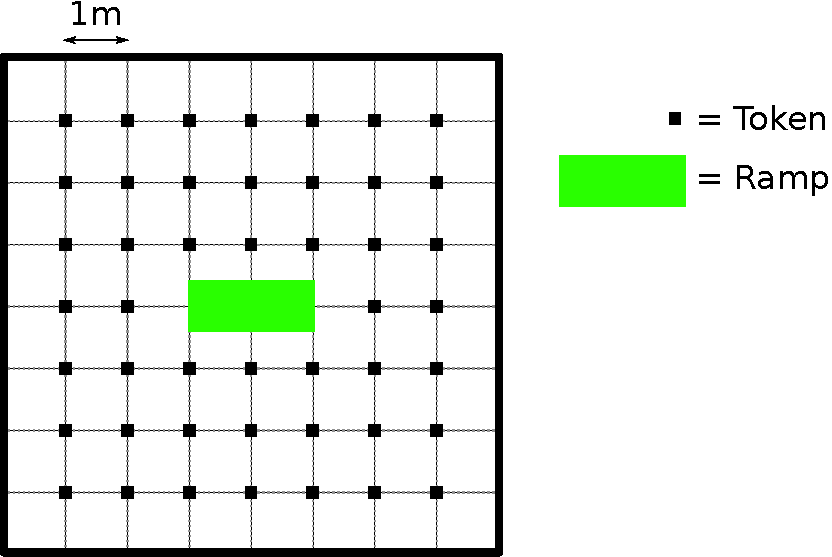
\includegraphics[keepaspectratio,width=0.7\textwidth]{./images/token-layout.pdf}
  \end{center}
  \caption{\label{fig:token-arrangement}Token arrangement in arena.}
\end{figure}
